
%(BEGIN_QUESTION)
% Copyright 2007, Tony R. Kuphaldt, released under the Creative Commons Attribution License (v 1.0)
% This means you may do almost anything with this work of mine, so long as you give me proper credit

Graph just the integral response of a {\it proportional+integral} controller with a proportional band of 50\% and an integral constant of 4 minutes per repeat to the following input conditions.  Assume a control action that is {\it reverse-acting}:

$$\includegraphics[width=15.5cm]{i01607x01.eps}$$

The time scale on the chart is minutes:seconds, and the PI algorithm is as follows:

$$m = K_p \left( e + {1 \over \tau_i} \int e \> dt \right) + b$$

\noindent
Where,

$m$ = Controller output (manipulated variable)

$K_p$ = Gain

$e$ = Error signal (SP$-$PV)

$\tau_i$ = Integral time constant

$b$ = Bias

\vskip 10pt

\underbar{file i01607}
%(END_QUESTION)





%(BEGIN_ANSWER)

$$\includegraphics[width=15.5cm]{i01607x02.eps}$$

First, let's convert the given tuning constants into direct-indicating units (gain instead of P.B., and rep/min instead of min/rep):
 
\vskip 10pt

Proportional band = 50\% ; Gain = 2
 
\vskip 10pt

4 minutes per repeat = 0.25 repeats per minute
 
\vskip 10pt
 
\noindent
Now, calculating the accumulated area under each deviation period:
 
\vskip 10pt
 
Integral action = $K_p {1\over \tau_i} \int e \> dt$
 
\vskip 10pt

Integral action = (gain)(repeats/min)(error-time product)
 
\vskip 10pt

Integral action = (2)(0.25/min)(2.5\%-min)
 
\vskip 10pt

Integral action = 1.25\%
 
\vskip 10pt

\noindent
{\it Output goes from 40\% to 38.75\%}

$$\includegraphics[width=15.5cm]{i01607x03.eps}$$

\filbreak 

Integral action = $K_p {1\over \tau_i} \int e \> dt$
 
\vskip 10pt

Integral action = (gain)(repeats/min)(error-time product)
 
\vskip 10pt

Integral action = (2)(0.25/min)(2.5\%-min)
 
\vskip 10pt

Integral action = 1.25\%
 
\vskip 10pt
 
\noindent
{\it Output goes from 38.75\% to 37.5\%}
 
$$\includegraphics[width=15.5cm]{i01607x04.eps}$$

\filbreak 

Integral action = $K_p {1\over \tau_i} \int e \> dt$
 
\vskip 10pt

Integral action = (gain)(repeats/min)(error-time product)
 
\vskip 10pt

Integral action = (2)(0.25/min)(2.5\%-min)
 
\vskip 10pt

Integral action = 1.25\%
 
\vskip 10pt
 
\noindent
{\it Output goes from 37.5\% to 38.75\%}
 
$$\includegraphics[width=15.5cm]{i01607x05.eps}$$

\filbreak 

Integral action = $K_p {1\over \tau_i} \int e \> dt$
 
\vskip 10pt

Integral action = (gain)(repeats/min)(error-time product)
 
\vskip 10pt

Integral action = (2)(0.25/min)(5\%-min)
 
\vskip 10pt

Integral action = 2.5\%
 
\vskip 10pt
 
\noindent
{\it Output goes from 38.75\% to 41.25\%}
 
$$\includegraphics[width=15.5cm]{i01607x06.eps}$$
 
\filbreak 

Integral action = $K_p {1\over \tau_i} \int e \> dt$
 
\vskip 10pt

Integral action = (gain)(repeats/min)(error-time product)
 
\vskip 10pt

Integral action = (2)(0.25/min)(5\%-min)
 
\vskip 10pt

Integral action = 2.5\%
 
\vskip 10pt

\noindent
{\it Output goes from 41.25\% to 43.75\%}
 
$$\includegraphics[width=15.5cm]{i01607x07.eps}$$

%(END_ANSWER)





%(BEGIN_NOTES)


%INDEX% Control, proportional + integral: graphing controller response

%(END_NOTES)


